\chapter{遅延聴覚フィードバックが身体運動に与える影響の調査}
本章では,第4章で開発されたシステムと第6章で決定された実験条件を用いて,遅延聴覚フィードバックが身体運動に及ぼす影響を聴力が正常な若年者および60代以上の高齢者に対して調査した結果について述べる.
「高齢者は若年者に比べて聴覚フィードバックの遅延に対する許容度が高い」という仮説を,4の倍数に達したときのみ遅延を発生させるシステムを用いて検証する.
第6章の予備実験により,4の倍数に達する直前の押下間隔と4の倍数に達した直後の押下間隔の差の二乗の平均値および中央値が遅延時間の増加に比例して増大すること,そして4の倍数に達したときの遅延が全体のボタン押下間隔のばらつきを拡大させるという可能性が示唆された.
これらの予備実験で得られた考察を基に,仮説の検証を行う.
\section{調査方法}
聴力の正常な若年者および高齢者を対象に行ったボタン押し課題による遅延聴覚フィードバックが身体運動に与える影響の調査の方法を以下に示す.
\begin{enumerate}
  \item 被験者に図4.1のシステムを用意する.
  \item 4章の手順1から手順2までに述べた方法によって,ボタン押し課題を実施する.
  \item ヘッドホンから出力される音声の遅延時間をランダムに変更して実験者がアプリケーション上で指定した回数だけ手順2を繰り返す.
  このとき,実験者が提示する回数は,7.2節で提示する遅延時間の種類によって異なる.
\end{enumerate}
\section{調査条件および調査対象}
遅延時間の提示順序は,最初に10[ms]を提示し,次に10[ms]以外の中からランダムに選択し提示する.
その後,残る遅延時間に10[ms]を加えたものをランダムに提示する.
提示する遅延時間の種類を表\ref{table:young_a},表\ref{table:young_b},表\ref{table:old_a}および表\ref{table:old_b}に示す.
本研究では,10, 30, 50, 70, 90, 110[ms]の6種類の遅延時間を用いた実験を実験Aとし,
10, 15, 20, 25, 35, 30, 40[ms]の7種類の遅延時間を用いた実験を実験Bと称する.
\begin{table}[tbp]
  \caption{若年者の実験Aにおける遅延時間の提示順}
  \label{table:young_a}
  \centering
  \begin{tabular}{lccc}
    \hline
    提示順 & 遅延時間 & 被験者数 & 年齢\\
     & [ms] & & $\bigl(平均 (最小-最大)\bigr)$\\
    \hline \hline
    提示順1  & 10, 30, 110, 10, 70, 90, 50  & 8 & $22.1\, (21-23)$\\
    提示順2  & 10, 70, 30, 110, 50, 90, 10  & 8 & $22.4\, (21-24)$\\
    提示順3  & 10, 110, 90, 50, 10, 30, 70  & 8 & $22.3\, (21-25)$\\
    提示順4  & 10, 50, 90, 10, 30, 70, 110  & 7 & $22.7\, (22-24)$\\
    提示順5  & 10, 30, 10, 50, 110, 70, 90  & 7 & $23.1\, (22-24)$
\\
    \hline
  \end{tabular}
\end{table}
\begin{table}[tbp]
  \caption{若年者の実験Bにおける遅延時間の提示順}
  \label{table:young_b}
  \centering
  \begin{tabular}{lccc}
    \hline
    提示順 & 遅延時間 & 被験者数 & 年齢\\
     & [ms] & & $\bigl(平均 (最小-最大)\bigr)$\\
    \hline \hline
    提示順1  & 10, 25, 35, 30, 40, 20, 10, 15  & 7 & $22.6\,(21-24)$\\
    提示順2  & 10, 15, 40, 10, 35, 25, 30, 20  & 7 & $22.9\,(21-25)$\\
    提示順3  & 10, 30, 25, 10, 40, 20, 35, 15  & 7 & $22.6\,(21-25)$\\
    提示順4  & 10, 30, 20, 10, 15, 35, 25, 40  & 7 & $22.1\,(20-24)$\\
    提示順5  & 10, 40, 10, 25, 30, 20, 15, 35  & 6 & $23.5\,(22-24)$
\\
    \hline
  \end{tabular}
\end{table}
\begin{table}[btp]
  \caption{高齢者の実験Aにおける遅延時間の提示順}
  \label{table:old_a}
  \centering
  \begin{tabular}{lccc}
    \hline
    提示順 & 遅延時間 & 被験者数 & 年齢\\
     & [ms] & & $\bigl(平均 (最小-最大)\bigr)$\\
    \hline \hline
    提示順1  & 10, 30, 110, 10, 70, 90, 50  & 8 & $63.5\, (60-70)$\\
    提示順2  & 10, 70, 30, 110, 50, 90, 10  & 8 & $70.1\, (61-77)$\\
    提示順3  & 10, 110, 90, 50, 10, 30, 70  & 8 & $68.4\, (63-77)$\\
    提示順4  & 10, 50, 90, 10, 30, 70, 110  & 9 & $70.2\, (61-82)$\\
    提示順5  & 10, 30, 10, 50, 110, 70, 90  & 8 & $74.1\, (68-83)$
\\
    \hline
  \end{tabular}
\end{table}
\begin{table}[btp]
  \caption{高齢者の実験Bにおける遅延時間の提示順}
  \label{table:old_b}
  \centering
  \begin{tabular}{lccc}
    \hline
    提示順 & 遅延時間 & 被験者数 & 年齢\\
     & [ms] & & $\bigl(平均 (最小-最大)\bigr)$\\
    \hline \hline
    提示順1  & 10, 25, 35, 30, 40, 20, 10, 15  & 8 & $70.0\,(60-80)$\\
    提示順2  & 10, 15, 40, 10, 35, 25, 30, 20  & 8 & $72.1\,(60-90)$\\
    提示順3  & 10, 30, 25, 10, 40, 20, 35, 15  & 8 & $67.9\,(60-88)$\\
    提示順4  & 10, 30, 20, 10, 15, 35, 25, 40  & 9 & $75.2\,(62-84)$\\
    提示順5  & 10, 40, 10, 25, 30, 20, 15, 35  & 8 & $73.1\,(65-80)$
\\
    \hline
  \end{tabular}
\end{table}
\newpage
\section{調査結果}
\subsection{観測値の分布}
% データの代表的な統計量,特に平均や標準偏差は,対象のデータ分布が正規分布に従っている場合にその真の特性を正確に反映する.
% したがって,遅延時間ごとに得られたボタンの押下時間間隔のデータが正規分布に従うかどうかを確認することが必要である.
% これにより,分散や標準偏差を用いてデータ分布のばらつきを評価することの妥当性を検討する.
% 帰無仮説を「ボタン押下時間間隔のデータの母集団の分布は,正規分布に従う」として,コルモゴロフ・スミルノフ検定を用いて,有意水準5%で観測値が正規分布に従うかどうかを検定する.
% 遅延時間に応じたボタンの押下時間間隔のデータのヒストグラムを図7.1,図7.2,図7.3,図7.4に示す.また,正規性の検定の結果を表7.1に記載する.
% 外れ値の除去は,被験者ごとに各遅延時間での観測値を
本節では,遅延時間ごとに得られたボタンの押下時間間隔のデータの分布を箱ひげ図を用いて示す.
箱ひげ図は,観測値の中央値,第1四分位数,第3四分位数を示すことで,データの分布状況および中心的傾向を効果的に視覚化する.
加えて,箱ひげ図に外れ値を示すことで,データのばらつきを直接的に評価することが可能となる.外れ値の算出は,以下の手順により行う.
\begin{enumerate}
  \item 各遅延時間におけるボタンの押下時間間隔のデータを,被験者ごとに集計する.
  \item 各遅延時間でのボタンの押下時間間隔のデータの中央値,第1四分位数,第3四分位数を算出する.
  \item 第3四分位数から第1四分位数を引いた値である四分位範囲(Interquartile Range, IQR)を計算する.
  \item (3)で求めたIQRを1.5倍し,この値を第三四分位数に加算および第一四分位数から減算した結果を上下の閾値と定める.
  \item 閾値内の最も遠いデータまで箱からひげを引く.
  \item 各データと閾値を比較し,(4)で求めた閾値の外にある値を全て外れ値とし,点で表す.
\end{enumerate}
これにより,データの基本的な統計的特徴を簡潔に表現し,後続の分析におけるデータの解釈を支援する.
図\ref{fig:110ms_Distribution_of_observations},図\ref{fig:40ms_Distribution_of_observations},
図\ref{fig:110ms_Distribution_of_observations_by_old}および図\ref{fig:40ms_Distribution_of_observations_by_old}に遅延時間ごとのボタンの押下時間間隔のデータの分布を示す.
これらの図より,それぞれの遅延時間でのボタンの押下時間間隔のデータには,一定数の外れ値が存在することがわかる.
したがって,本研究では外れ値を除外したデータを用いて分析を行う.
この方法により,これから行う分析において,外れ値の影響を排除し,データの適切な評価を行うことができる.

\begin{figure}[tbp]
  \centering
  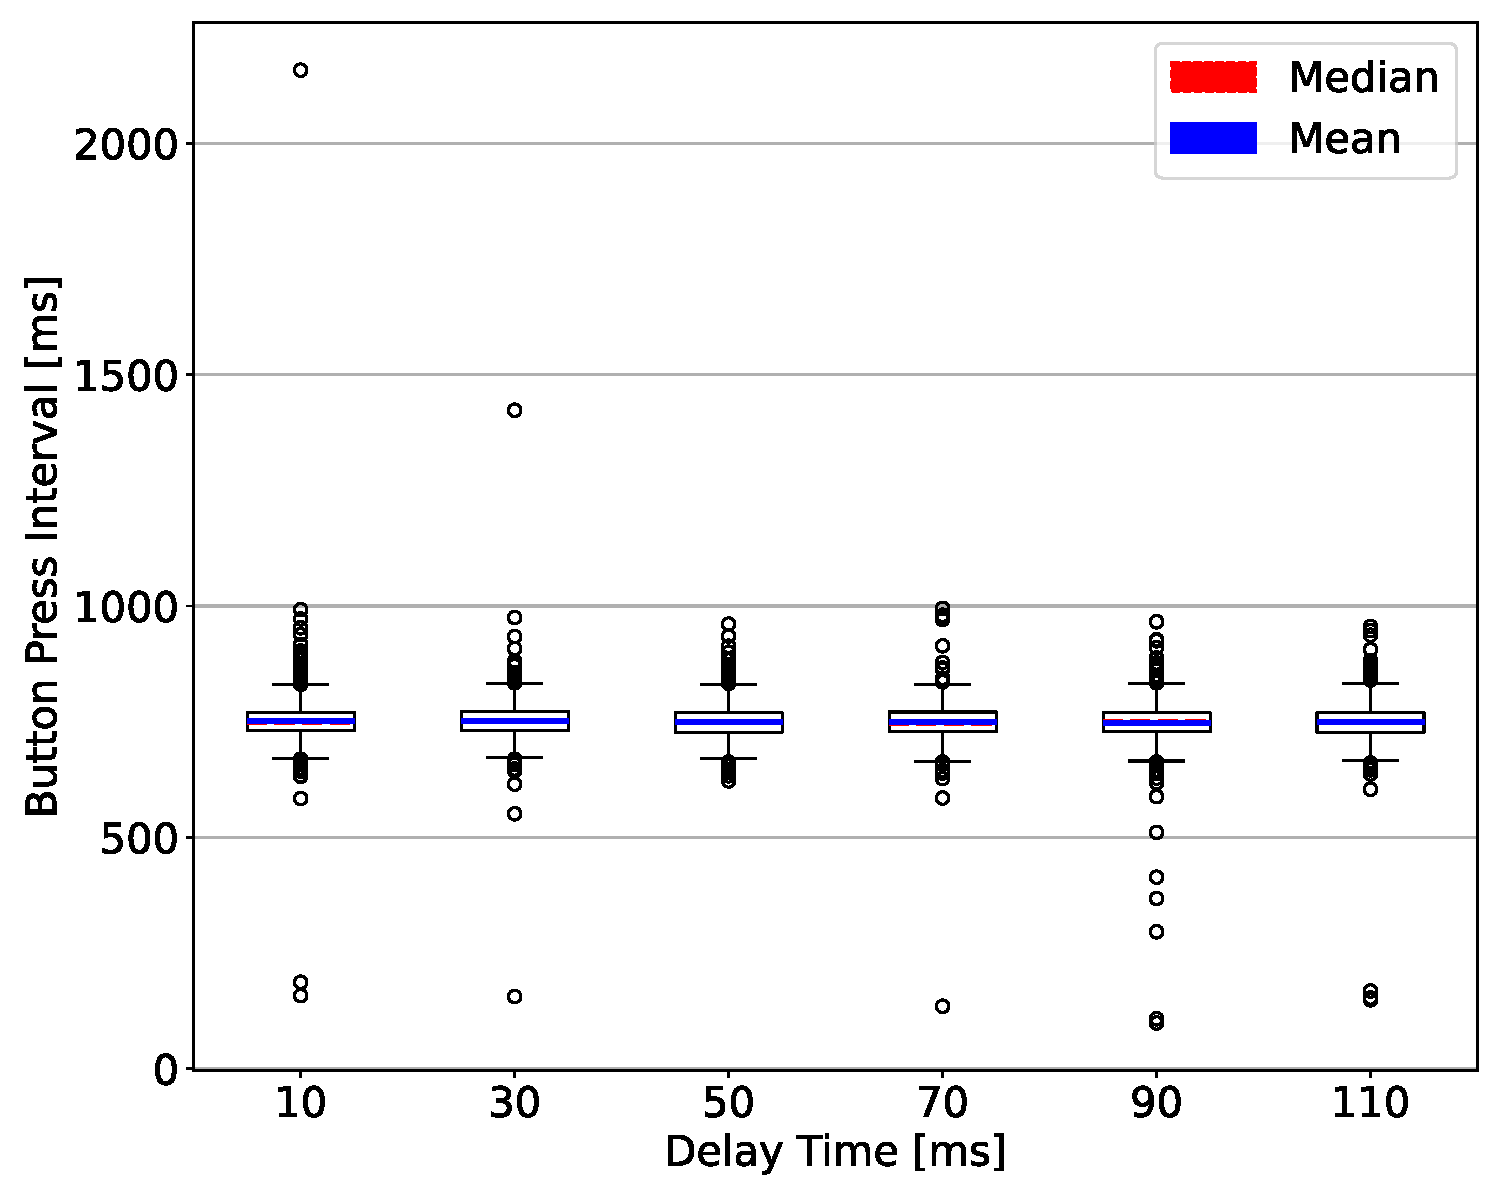
\includegraphics[scale=0.4]{figures/Honbann/BOXPLOT/young_110_boxplot.pdf}
  \caption{実験Aにおける遅延時間ごとの若年者のデータの分布}
  \label{fig:110ms_Distribution_of_observations}
\end{figure}
\begin{figure}[tbp]
  \centering
  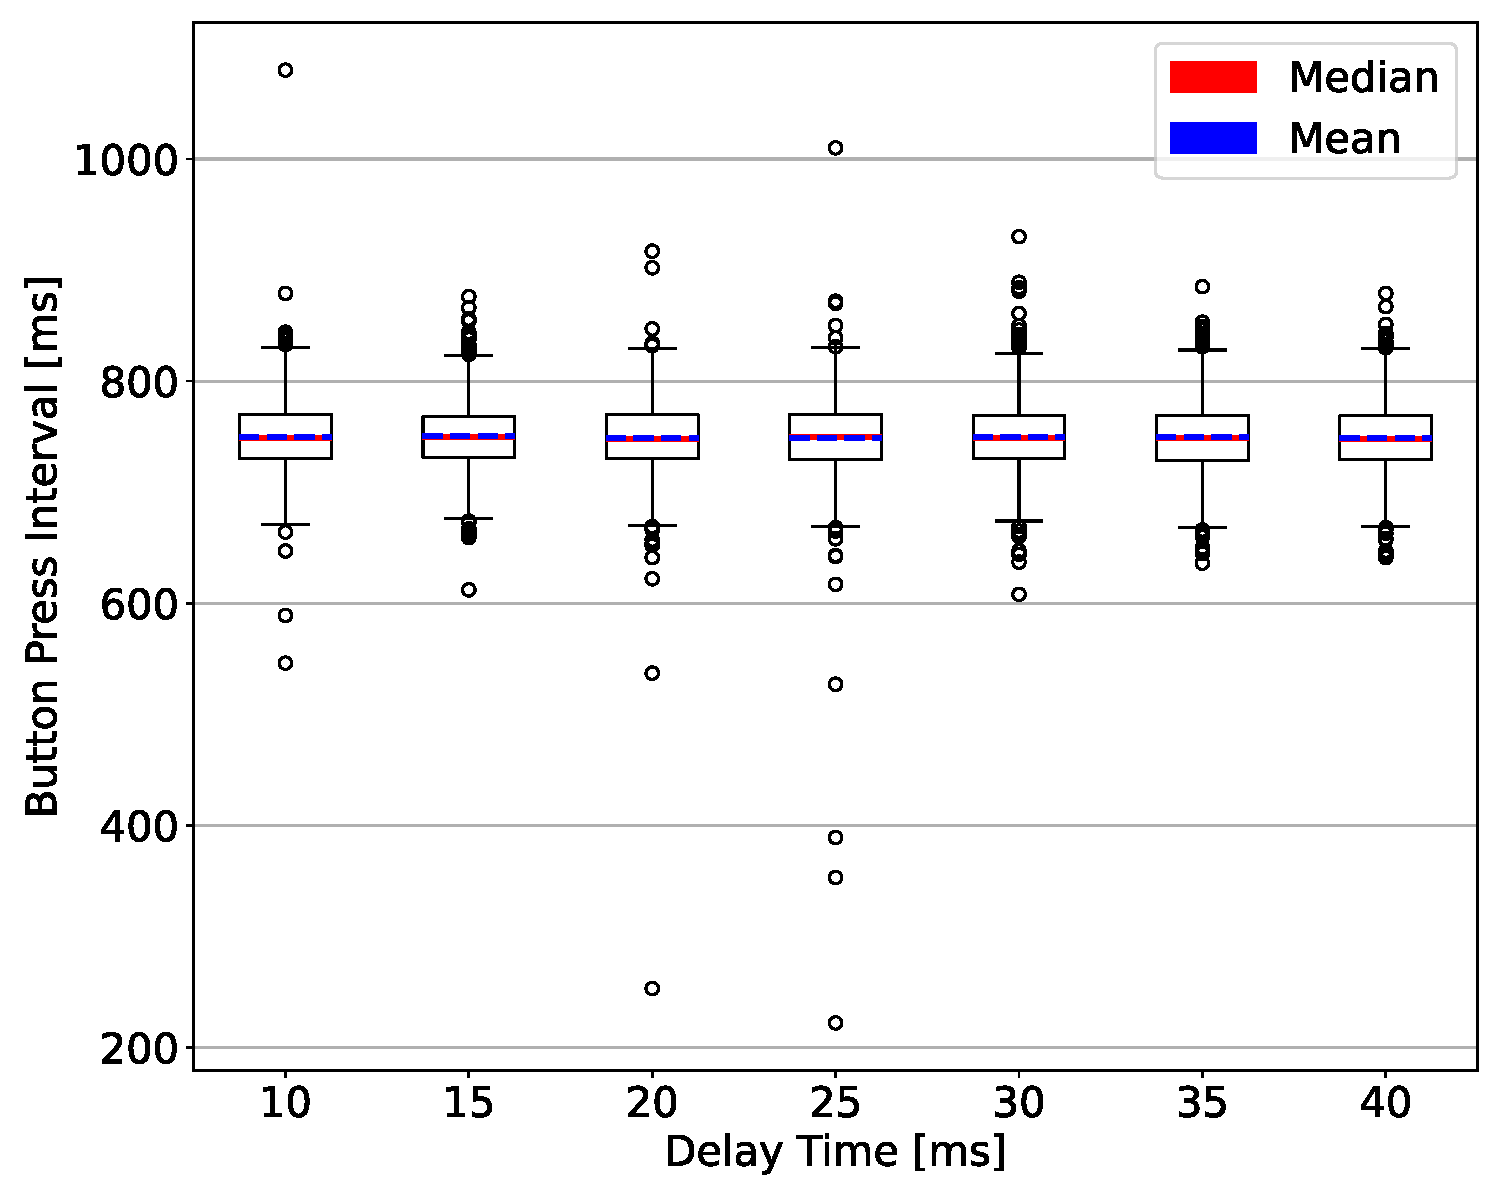
\includegraphics[scale=0.4]{figures/Honbann/BOXPLOT/young_40_boxplot.pdf}
  \caption{実験Bにおける遅延時間ごとの若年者のデータの分布}
  \label{fig:40ms_Distribution_of_observations}
\end{figure}
\begin{figure}[tbp]
  \centering
  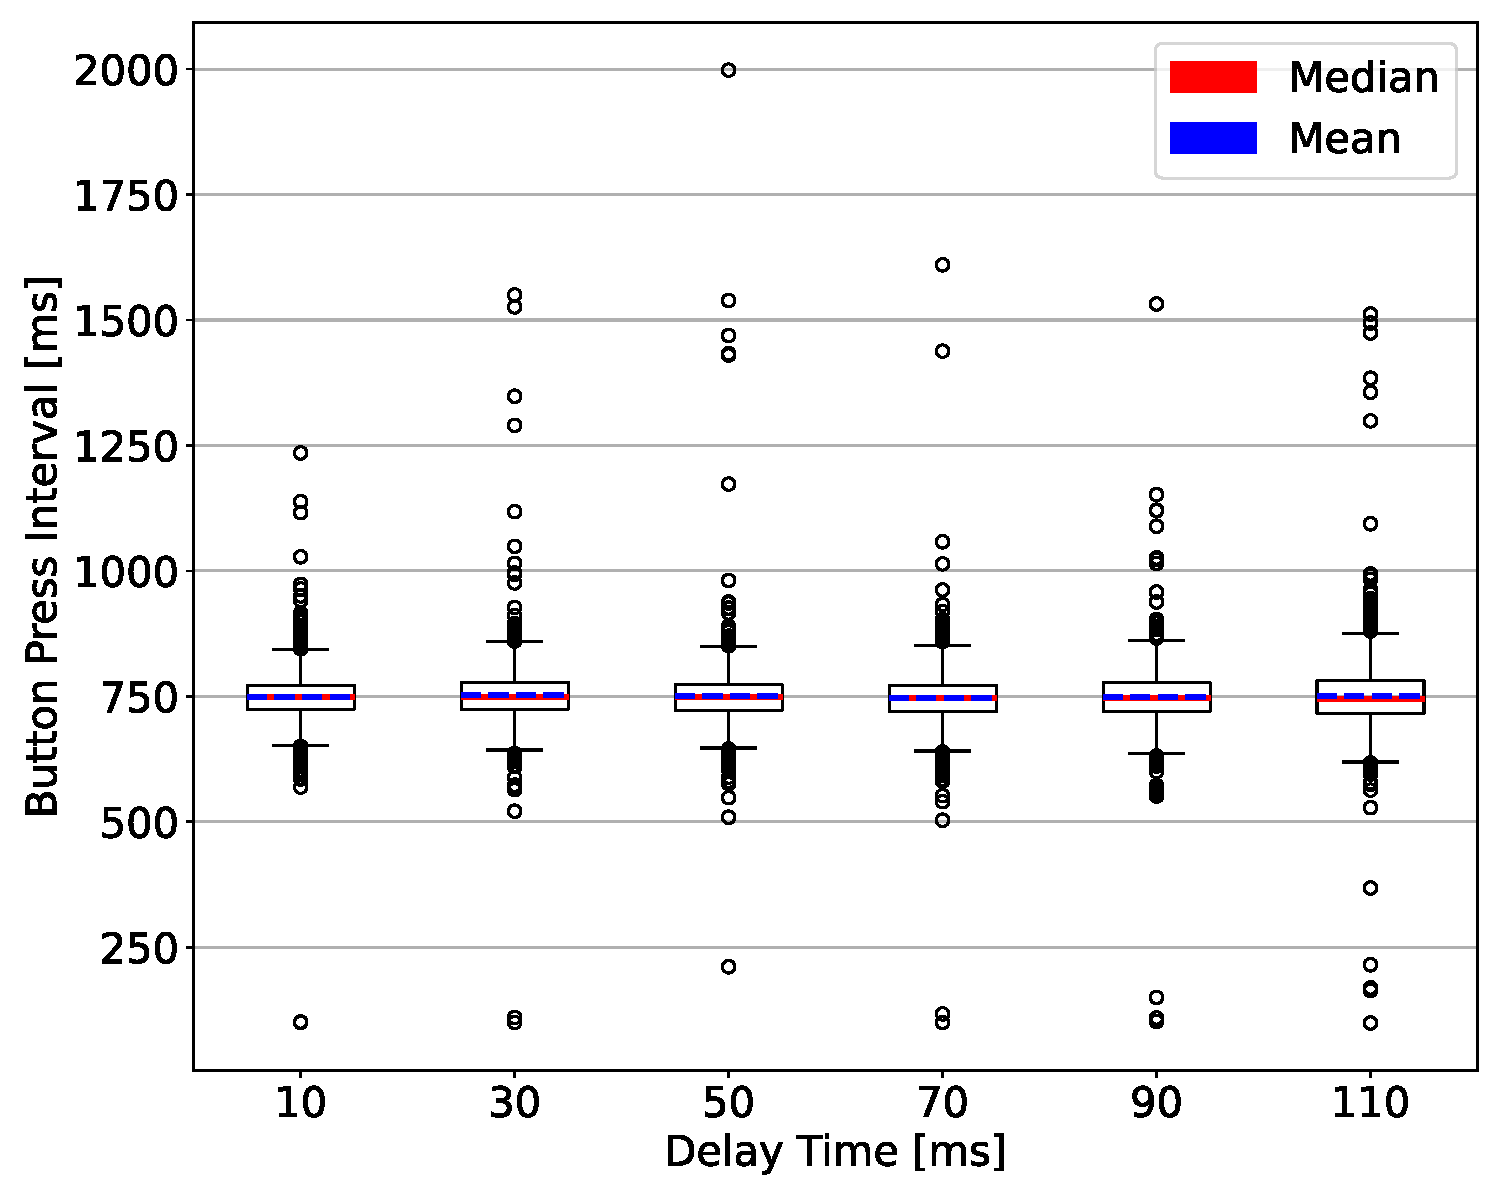
\includegraphics[scale=0.4]{figures/Honbann/BOXPLOT/old_110_boxplot.pdf}
  \caption{実験Aにおける遅延時間ごとの高齢者のデータの分布}
  \label{fig:110ms_Distribution_of_observations_by_old}
\end{figure}
\begin{figure}[tbp]
  \centering
  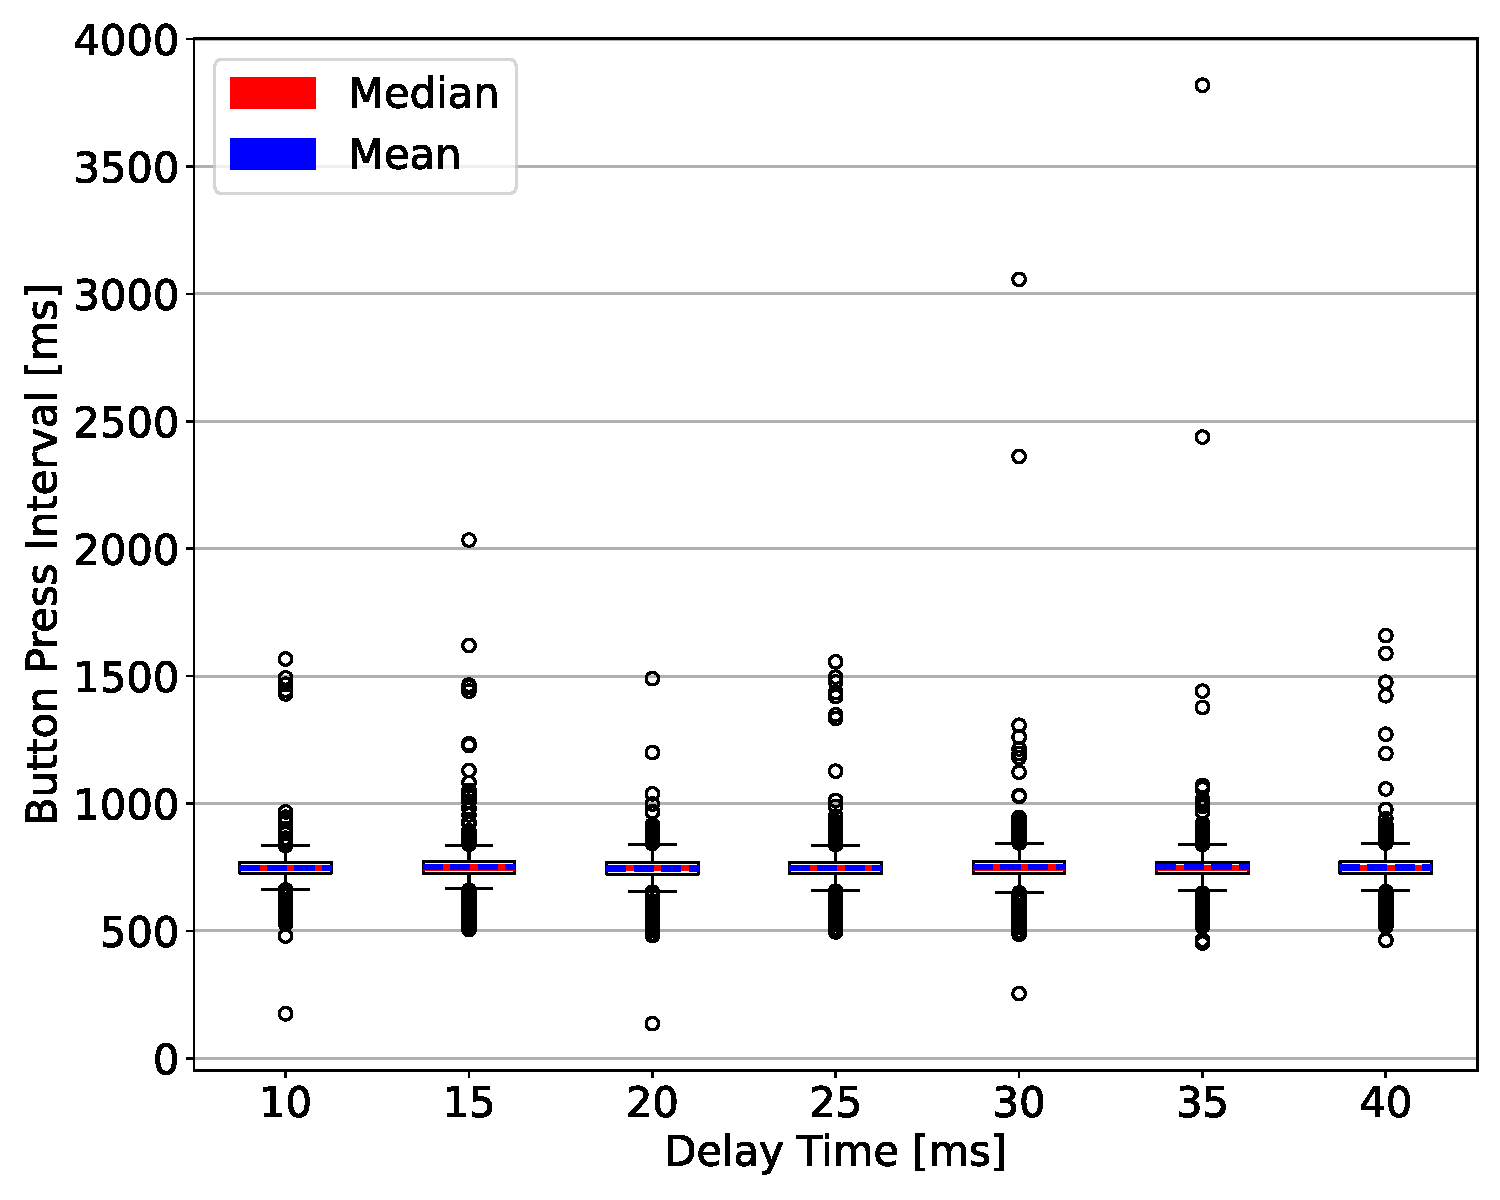
\includegraphics[scale=0.4]{figures/Honbann/BOXPLOT/old_40_boxplot.pdf}
  \caption{実験Bにおける遅延時間ごとの高齢者のデータの分布}
  \label{fig:40ms_Distribution_of_observations_by_old}
\end{figure}
\newpage
% 結果の考察
\subsection{遅延時間と評価指標の関係}
本節では,7.3.1項で説明した方法によりデータの外れ値を除去した後の遅延聴覚フィードバックが身体運動に与える影響の調査結果を標本全体の分散,
遅延直前および直後の押下時間間隔の差の二乗の平均値(Mean Squared Error, MSE),遅延直前および直後の押下間隔の差の中央値(Median Squared Error, MedSE)
の3つの評価指標を用いて示す.
遅延時間と評価値の関係が若年者と高齢者で異なるかどうかを検証するために,若年者と高齢者それぞれの結果を同一グラフ上に表示し,比較する.
図\ref{fig:Var_110ms_Sa_Sb},図\ref{fig:Var_110ms_Sc}に実験Aにおける遅延時間と分散の関係,
図\ref{fig:Var_40ms_Sa_Sb},図\ref{fig:Var_40ms_Sc}に実験Bにおける遅延時間と分散の関係,
図\ref{fig:Normalized-Var_110ms_SaSbSc},図\ref{fig:Normalized-Var_40ms_SaSbSc}に実験A,実験Bにおける遅延時間と分散の関係において,遅延時間が10[ms]時の評価値を基準に正規化した場合の結果を示す.
図\ref{fig:110ms_MSE_MedSE},図\ref{fig:Normalized_110ms_MSE_MedSE}にMSEおよびMedSEの結果を,
図\ref{fig:40ms_MSE_MedSE},図\ref{fig:Normalized_40ms_MSE_MedSE}にMSEおよびMedSEの結果を遅延時間が10[ms]時の評価値で正規化した場合の結果を示す.

%%%%%%%%%%%%%%%%%%%%%%%%%%%%%%%
% 実験A
%%%%%%%%%%%%%%%%%%%%%%%%%%%%%%%
はじめに,実験Aにおける結果について述べる.
実験Aの結果において,ボタンの押下時間間隔全体の分散を評価値とする指標によれば,正規化されたデータでは若年者と高齢者の反応に顕著な差異が見られる.
若年者は,一貫して評価値が緩やかに増加するのに対し,高齢者は110[ms]を境に分散が大幅に増加することが示された.
また,実験AにおけるMSEおよびMedSEによる評価からも,遅延時間の増加に伴い,若年者と高齢者双方の評価値に増加の傾向が確認された.
この結果は,ボタン押し課題で提供される聴覚フィードバックの遅延が長くなるにつれて,遅延聴覚フィードバックの影響がより顕著になることを示唆している.
若年者は遅延時間の増加に対して比較的均一な反応を示したが,対照的に高齢者は70[ms]まで比較的緩やかな増加を見せた後,90[ms], 110[ms]の遅延時間において顕著な反応の増加を示した.
これは,高齢者がある程度の遅延には許容度を持つことを示唆しており,遅延時間が110[ms]に達した際には,若年者との差異が特に明確になった.
これらの結果から,高齢者が若年者と比較して聴覚フィードバックの遅延に対する許容度が高い可能性が示され,結果として遅延時間の増加に対する高齢者の感知の鈍さが推測される.
さらに,高齢者の評価値が若年者と比較して一貫性に欠けることからも,高齢者が遅延に対して鈍感である可能性も示唆される.

%%%%%%%%%%%%%%%%%%%%%%%%%%%%%%%
% 実験B
%%%%%%%%%%%%%%%%%%%%%%%%%%%%%%
次に,実験Bにおける結果について述べる.
実験Bにおいてもボタン押し課題の押下時間間隔全体の分散を通じて分析した結果,若年者と高齢者での間で異なる傾向が観察された.
正規化されたデータに基づく評価では,10[ms]から40[ms]の遅延時間帯において,若年者の分散は一貫して低い水準を維持しながらも緩やかに増加しているのに対し,
高齢者は遅延時間と評価値の間に一貫した関係が認められない.
% このことは,若年者が遅延時間の増加に対して一貫性を維持しやすく,高齢者は,遅延時間の増加に対して一貫性を維持することが困難であることを示唆している.
非正規化されたデータに基づく分析でも,高齢者は遅延時間に対して比較的一貫した分散の値を示しているが,若年者に比べて全体的に高い分散値を記録している.
これらのことは,高齢者が遅延時間の増加に対して若年者よりも鈍感であることを示唆し,逆に若年者が遅延時間の変化に対してより敏感である可能性を示している.
また,MSEおよびMedSEによる評価では,10[ms]から40[ms]の比較的短い遅延時間帯において,若年者における評価値が緩やかに増加する傾向が認められ,
若年者が遅延時間の増加に対して比較的敏感であること,そして遅延聴覚フィードバックによる影響をより感じやすいことを示唆している.
一方で,高齢者においては,遅延時間と評価値の間に一貫した関係が見出されず,遅延に対する感受性の低さが示唆される.
% 特に,高齢者群の評価値は遅延時間の変化に対して一定のばらつきを示しており,これは高齢者が遅延に対して鈍感である可能性を示している.

%%%%%%%%
% 結び
%%%%%%%%
以上の結果をまとめると,10[ms]から40[ms]の短い遅延時間帯における観察結果から,若年者の反応は遅延時間の増加に伴い緩やかに増加する傾向にあるが,
高齢者の反応には一貫した関係が認められないことが示された.このことは,若年者が遅延に対して敏感であり,一方で高齢者が遅延時間に対してある程度の
許容度を持っていることを示唆している.
一方,遅延時間を10[ms]から110[ms]に拡大した場合,特に90[ms]を超える長い遅延時間帯における高齢者の反応に大幅な増加が観察され,高齢者が遅延時間の
増加に対して比較的鈍感であるものの,90[ms]を超えるとタスクの一貫性を保つことが困難になることが示された.
若年者も長い遅延時間において,反応の増加を示したが,この増加は高齢者ほど急激ではなかった.
これらの結果は,遅延時間が増加するにつれて若年者と高齢者の反応の差異が顕著になることを示し,
若年者は短い遅延時間帯でも遅延を感じやすく,高齢者は長い遅延時間において特に顕著な反応を示したことを明らかにする.
さらに,遅延時間に対する年齢別の感受性の違いは,遅延聴覚フィードバックにおける効果を最大化するための異なるアプローチの
重要性を協調するものと思われる.
% 高齢者の遅延に対する許容度が高いという結果は,遅延聴覚フィードバックの適用において,年齢に応じた遅延時間の設定が必要であることを示唆している.
% 遅延時間の増加に対する若年者の反応の敏感さは,聴覚処理能力が発達していることを示しつつも,遅延聴覚フィードバックの影響を受けやすいという特性を持っていることを明らかにしている.
% これは,遅延処理能力や注意制御の能力において,年齢による差異が存在することが示唆される.
% 高齢者の評価値が一貫して大きいことから高齢者が若年者と比較して一貫性のあるリズムでボタンを押すことが難しく,注意制御の能力や運動制御の能力において,年齢による差異が存在することが示唆される.
%%%%%%%
% 正規化なし
%%%%%%%
\begin{figure}[tbp]
  \centering
  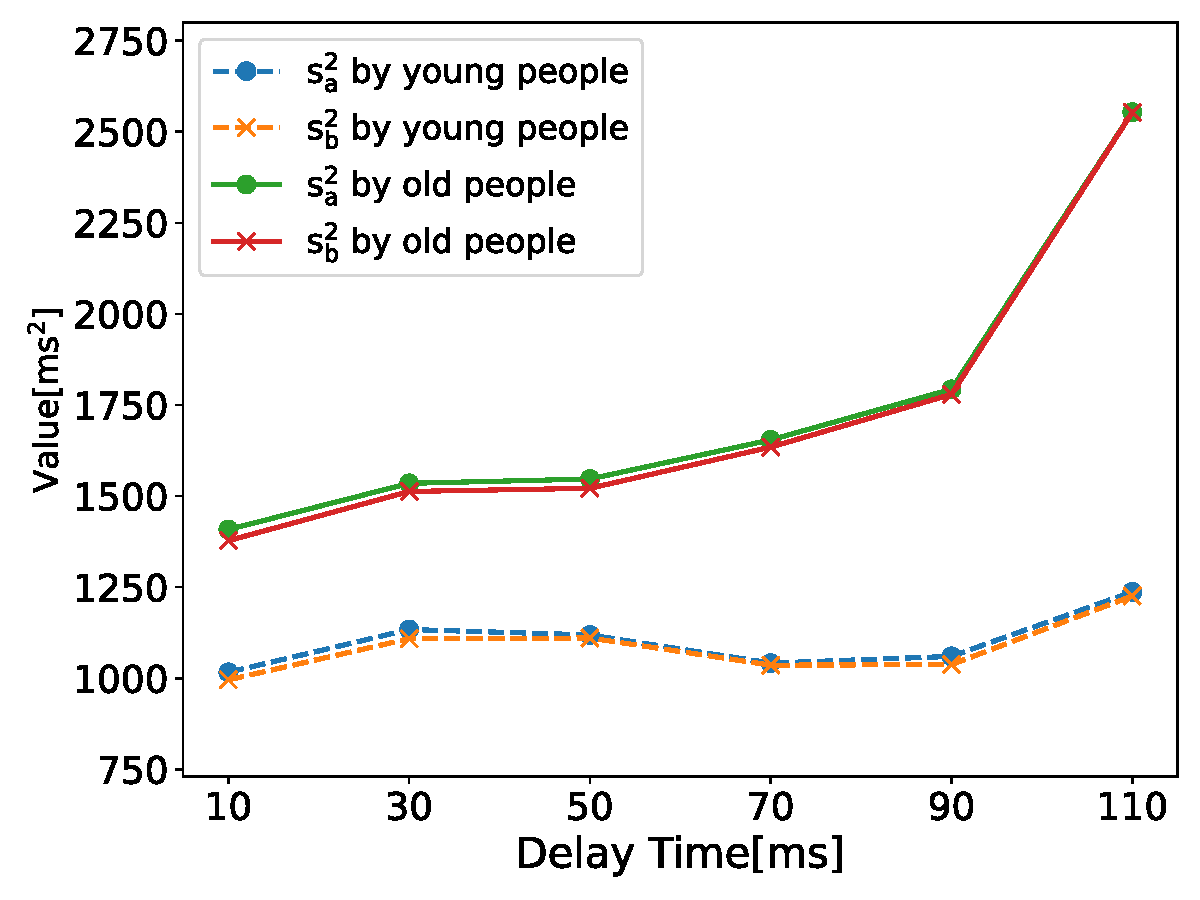
\includegraphics[scale=0.5]{figures/Honbann/Comparison_young_old/110_var_SaSb.pdf}
  \caption{実験Aにおける若年者と高齢者の分散の比較1}
  \label{fig:Var_110ms_Sa_Sb}
\end{figure}
\begin{figure}[tbp]
  \centering
  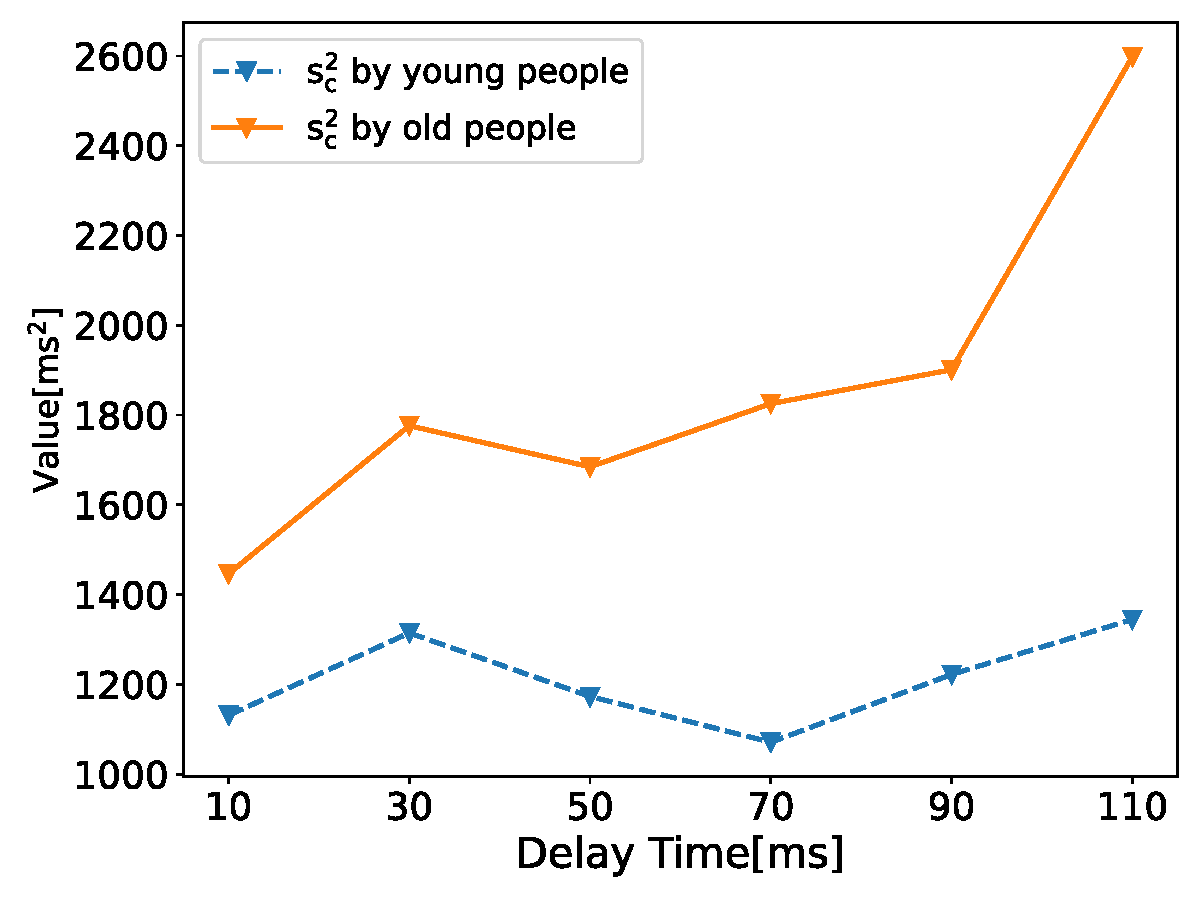
\includegraphics[scale=0.5]{figures/Honbann/Comparison_young_old/110_var_Sc.pdf}
  \caption{実験Aにおける若年者と高齢者の分散の比較2}
  \label{fig:Var_110ms_Sc}
\end{figure}

\begin{figure}[tbp]
  \centering
  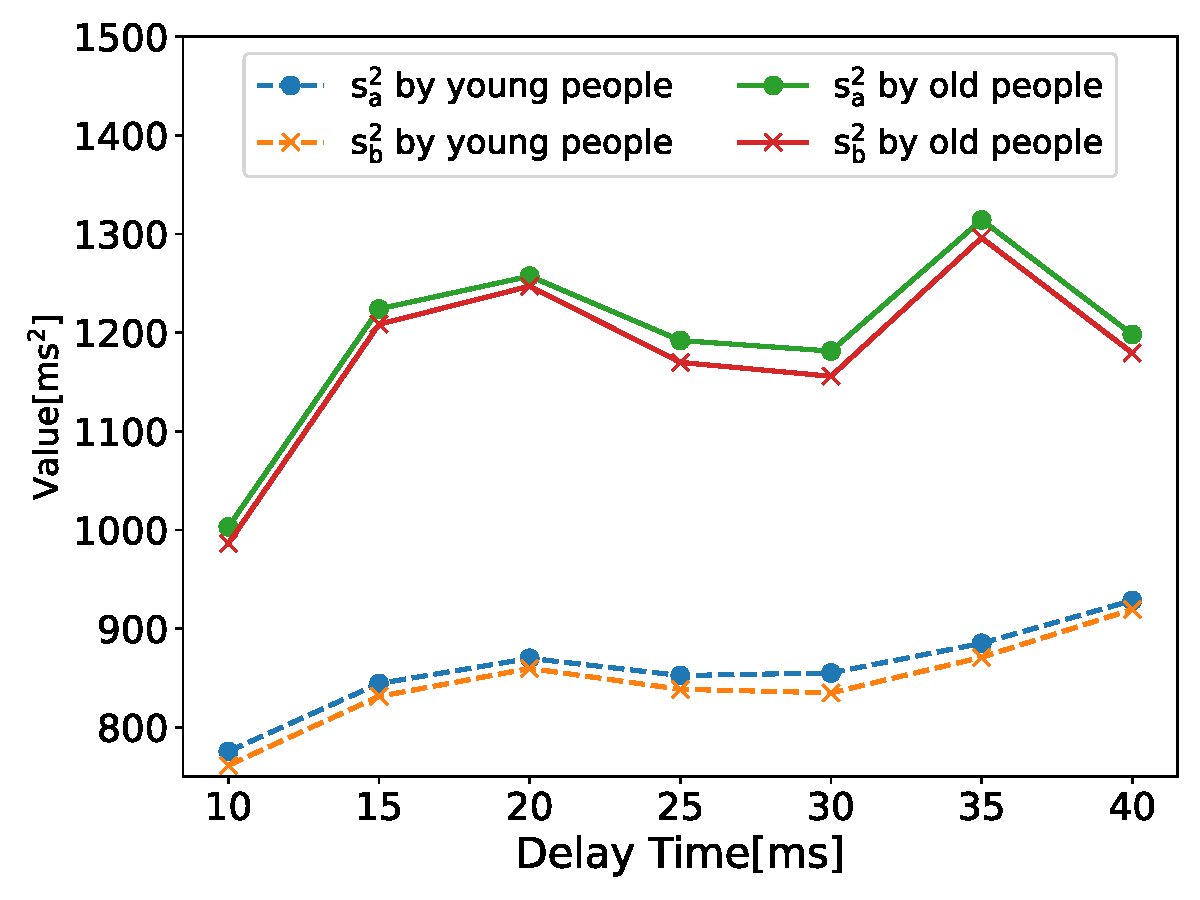
\includegraphics[scale=0.5]{figures/Honbann/Comparison_young_old/40_var_SaSb.pdf}
  \caption{実験Bにおける若年者と高齢者の分散の比較1}
  \label{fig:Var_40ms_Sa_Sb}
\end{figure}

\begin{figure}[tbp]
  \centering
  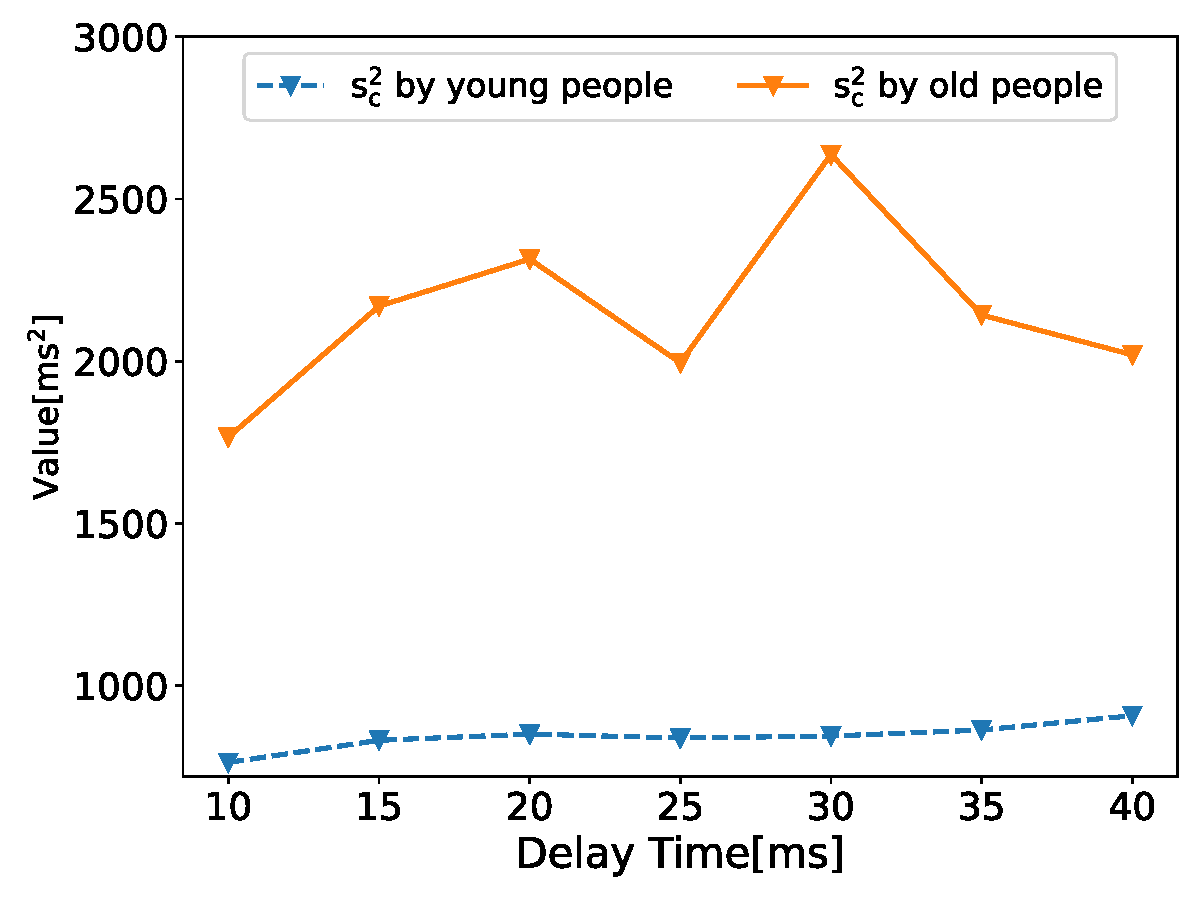
\includegraphics[scale=0.5]{figures/Honbann/Comparison_young_old/40_var_Sc.pdf}
  \caption{実験Bにおける若年者と高齢者の分散の比較2}
  \label{fig:Var_40ms_Sc}
\end{figure}

%%%%%%%
% 正規化あり
%%%%%%%
\begin{figure}[tbp]
  \centering
  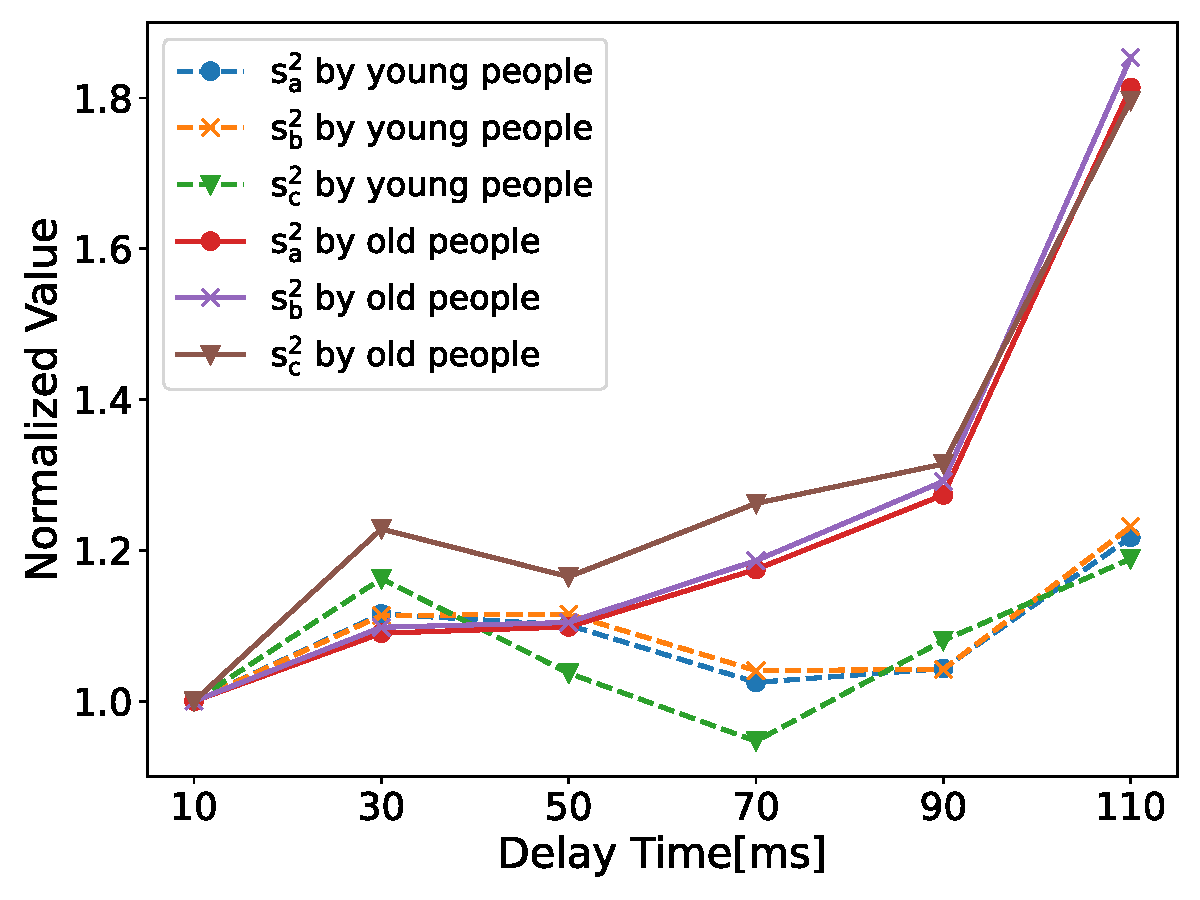
\includegraphics[scale=0.5]{figures/Honbann/Comparison_young_old/110_var_normalized.pdf}
  \caption{実験Aにおける若年者と高齢者の正規化後の評価値の比較}
  \label{fig:Normalized-Var_110ms_SaSbSc}
\end{figure}

\begin{figure}[tbp]
  \centering
  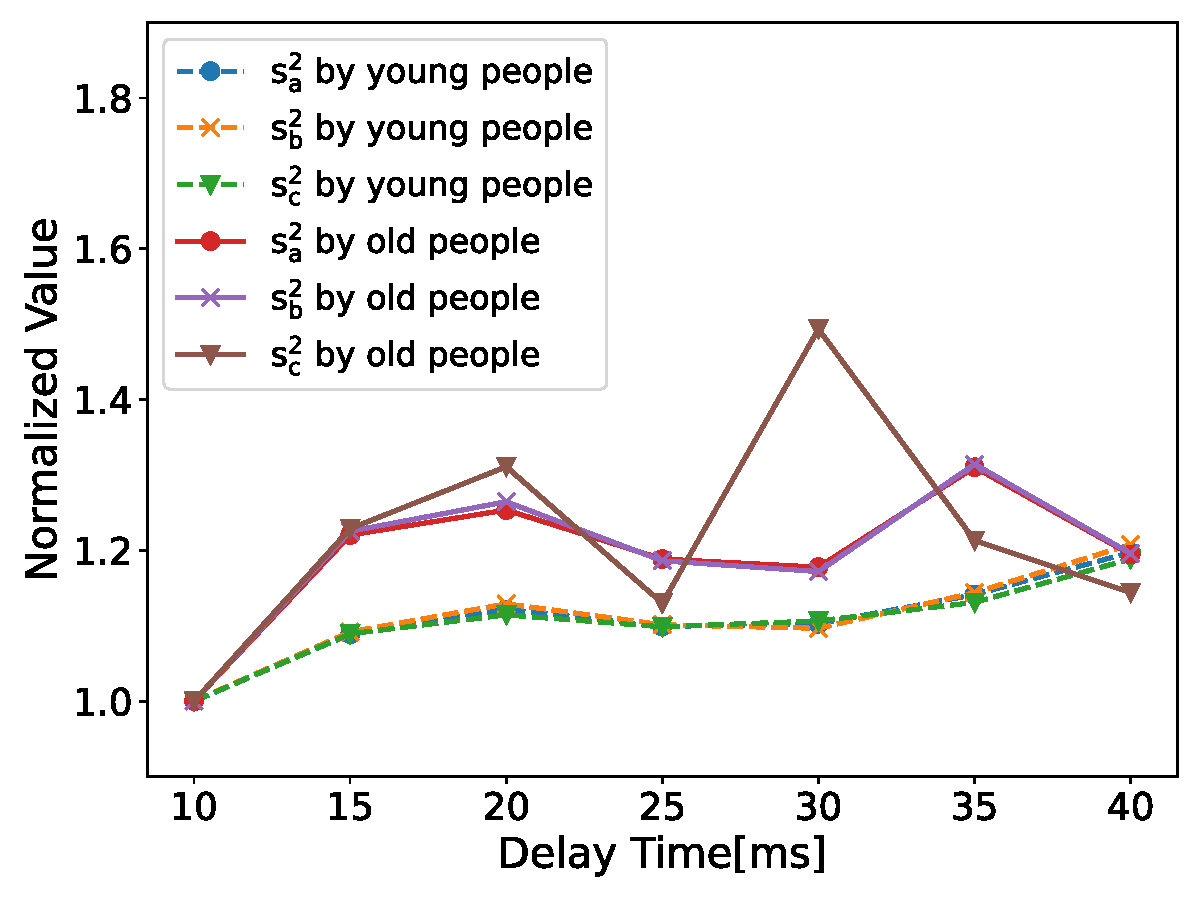
\includegraphics[scale=0.5]{figures/Honbann/Comparison_young_old/40_var_normalized.pdf}
  \caption{実験Bにおける若年者と高齢者の正規化後の評価値の比較}
  \label{fig:Normalized-Var_40ms_SaSbSc}
\end{figure}
 %%%%%%%%%%%%%%%%%%%%%%% ここまで

\begin{figure}[tbp]
  \centering
  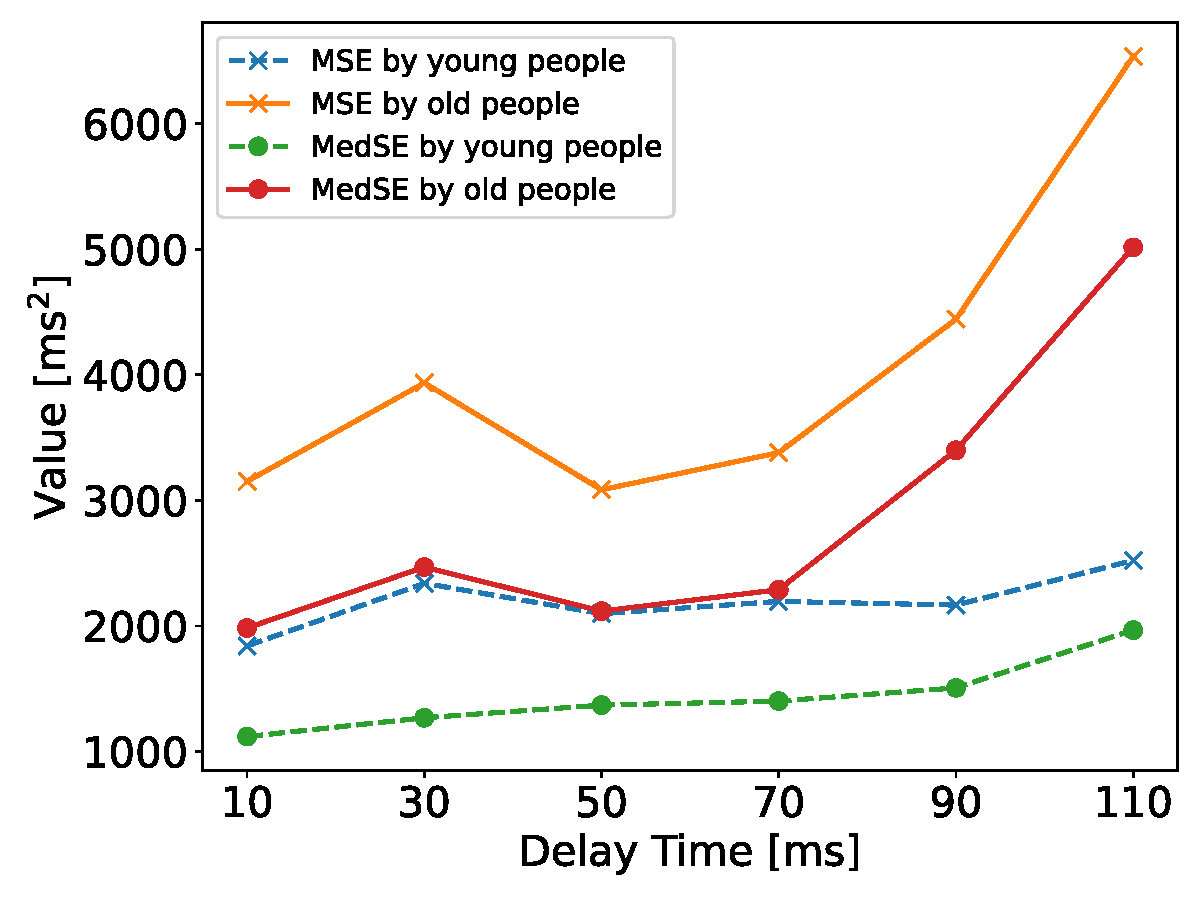
\includegraphics[scale=0.5]{figures/Honbann/Comparison_young_old/110_MSE-MedSE.pdf}
  \caption{実験Aにおける若年者と高齢者のMSEとMedSEの比較}
  \label{fig:110ms_MSE_MedSE}
\end{figure}
\begin{figure}[tbp]
  \centering
  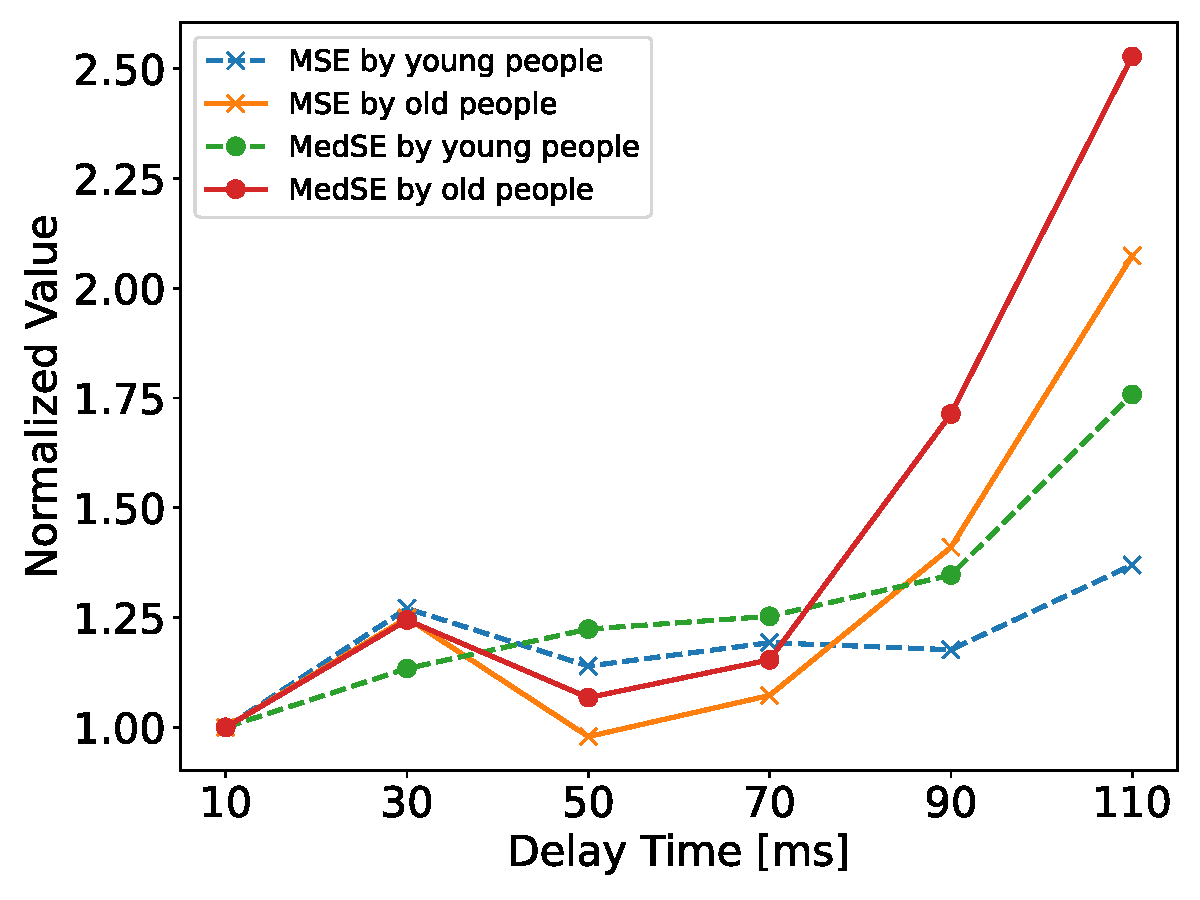
\includegraphics[scale=0.5]{figures/Honbann/Comparison_young_old/110_MSE-MedSE_normalized.pdf}
  \caption{実験Aにおける若年者と高齢者の正規化後のMSEとMedSEの比較}
  \label{fig:Normalized_110ms_MSE_MedSE}
\end{figure}
\begin{figure}[tbp]
  \centering
  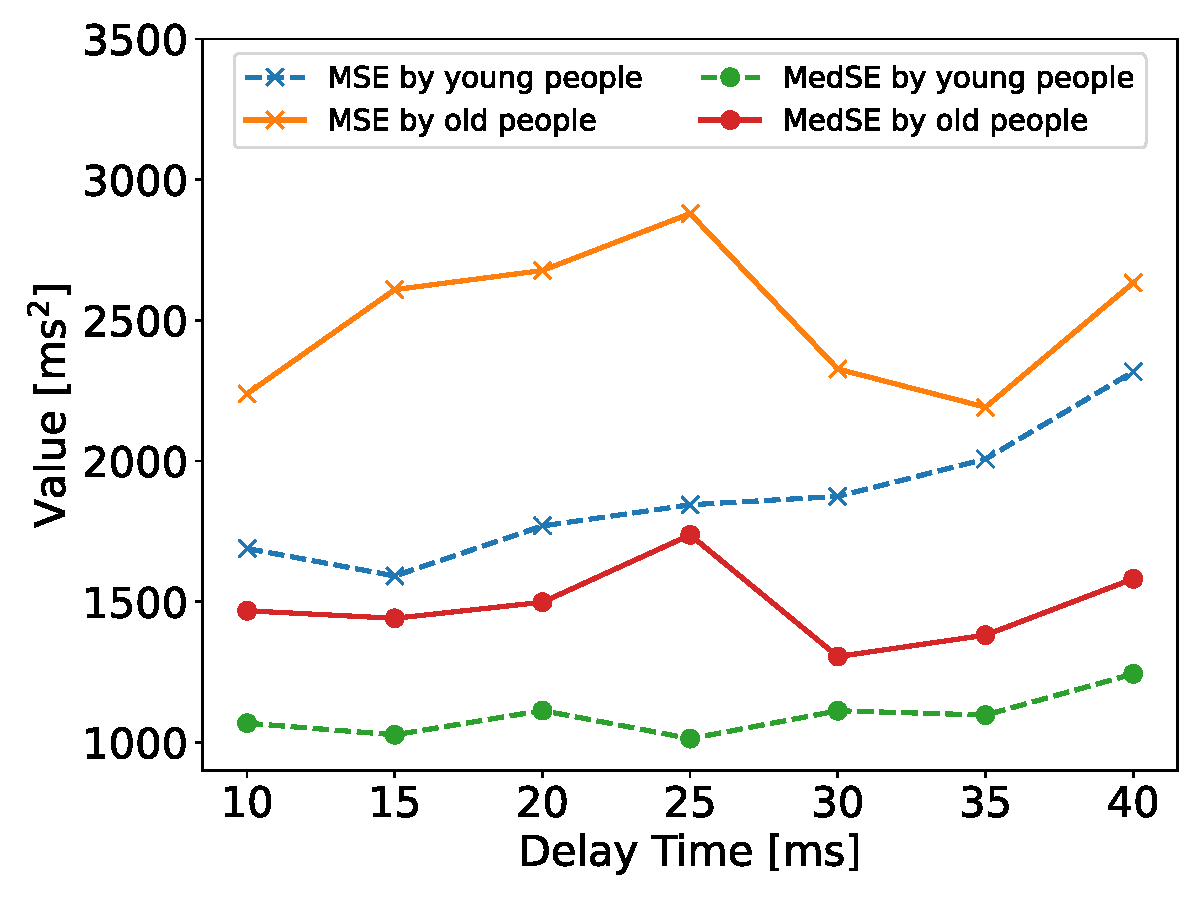
\includegraphics[scale=0.5]{figures/Honbann/Comparison_young_old/40_MSE-MedSE.pdf}
  \caption{実験Bにおける若年者と高齢者のMSEとMedSEの比較}
  \label{fig:40ms_MSE_MedSE}
\end{figure}

\begin{figure}[tbp]
  \centering
  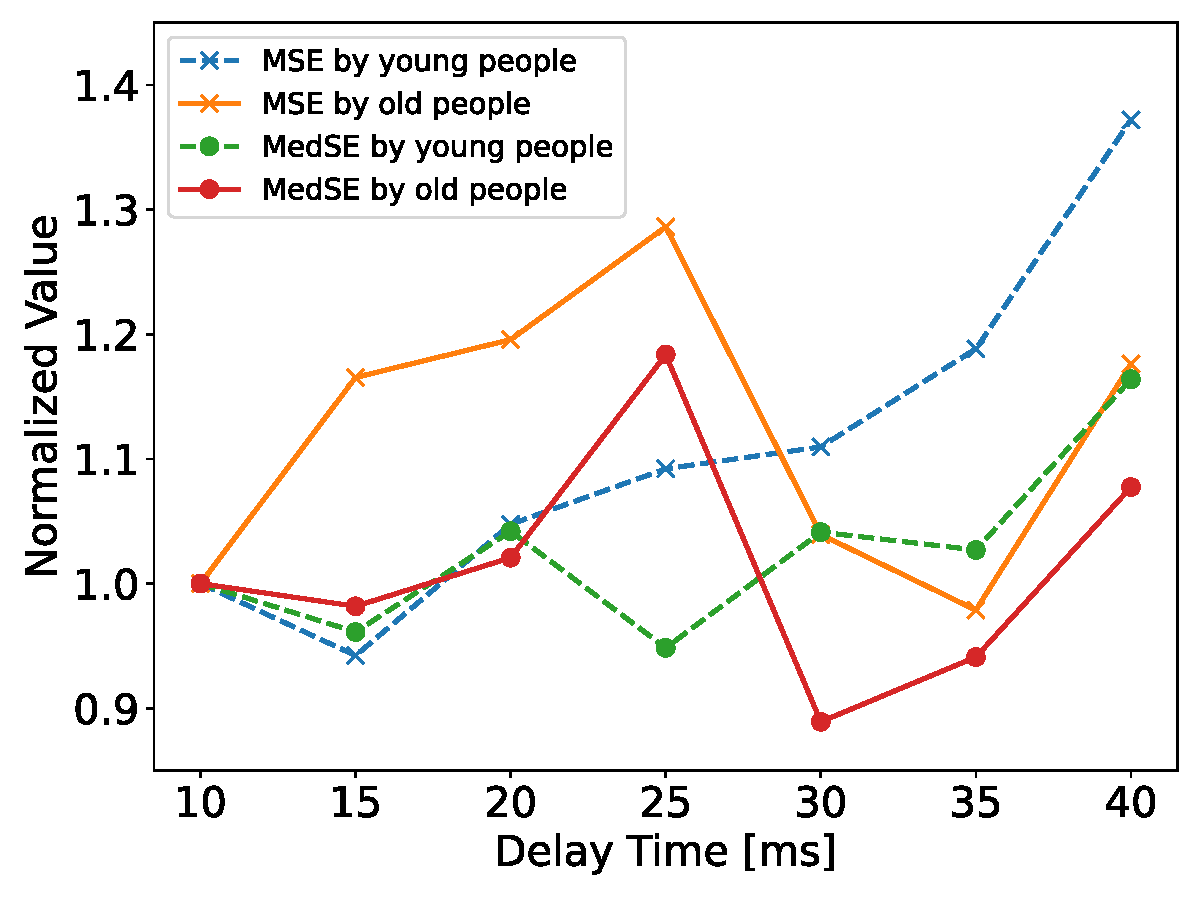
\includegraphics[scale=0.5]{figures/Honbann/Comparison_young_old/40_MSE-MedSE_normalized.pdf}
  \caption{実験Bにおける若年者と高齢者の正規化後のMSEとMedSEの比較}
  \label{fig:Normalized_40ms_MSE_MedSE}
\end{figure}